\begin{marginfigure}[1cm]
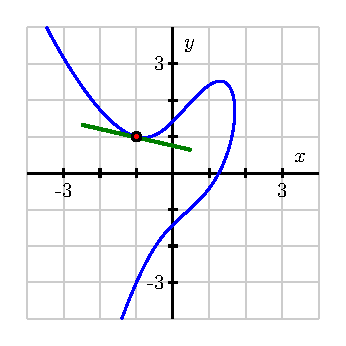
\includegraphics{figures/2_7_Ex1.eps}
\caption{The curve $x^3 + y^2 - 2xy = 2$.} \label{fig:2-7_Eg1}
\end{marginfigure}

\begin{example} \label{Ex:2.7.Eg1}
For the curve given implicitly by $x^3 + y^2 - 2xy = 2$, shown in Figure~\ref{fig:2-7_Eg1}, find the slope of the tangent line at $(-1,1)$.

\solution We begin by differentiating the curve's equation implicitly.  Taking the derivative of each side with respect to $x$,
$$\frac{d}{dx}\left[ x^3 + y^2 - 2xy \right] = \frac{d}{dx} \left[ 2 \right],$$
by the sum rule and the fact that the derivative of a constant is zero, we have
$$\frac{d}{dx}[x^3] + \frac{d}{dx}[y^2] - \frac{d}{dx}[2xy] = 0.$$
For the three derivatives we now must execute, the first uses the simple power rule, the second requires the chain rule (since $y$ is an implicit function of $x$), and the third necessitates the product rule (again since $y$ is a function of $x$).  Applying these rules, we now find that
$$3x^2 + 2y\frac{dy}{dx} - [2x \frac{dy}{dx} + 2y] = 0.$$
Remembering that our goal is to find an expression for $\frac{dy}{dx}$ so that we can determine the slope of a particular tangent line, we want to solve the preceding equation for $\frac{dy}{dx}$.  To do so, we get all of the terms involving $\frac{dy}{dx}$ on one side of the equation and then factor.  Expanding and then subtracting $3x^2 - 2y$ from both sides, it follows that
$$2y\frac{dy}{dx} - 2x \frac{dy}{dx}= 2y - 3x^2.$$
Factoring the left side to isolate $\frac{dy}{dx}$, we have
$$\frac{dy}{dx}(2y - 2x) = 2y - 3x^2.$$
Finally, we divide both sides by $(2y - 2x)$ and conclude that
$$\frac{dy}{dx} = \frac{2y-3x^2}{2y-2x}.$$
Here again, the expression for $\frac{dy}{dx}$ depends on both $x$ and $y$.  To find the slope of the tangent line at $(-1,1)$, we substitute this point in the formula for $\frac{dy}{dx}$, using the notation
$$ \left. \frac{dy}{dx} \right|_{(-1,1)} = \frac{2(1)-3(-1)^2}{2(1)-2(-1)} = -\frac14.$$
This value matches our visual estimate of the slope of the tangent line shown in Figure~\ref{fig:2-7_Eg1}.

%We now proceed to find all points on the curve where the tangent line is horizontal.  To have a horizontal tangent line, it must be the case that $\frac{dy}{dx} = 0$.  Taking the formula we derived for $\frac{dy}{dx}$, for this expression to be zero, its numerator must be zero, and thus $2y - 3x^2 = 0$, so that $y = \frac{3}{2}x^2.$  This tells us that at any point on the curve $x^3 + y^2 - 2xy = 2$ where $y = \frac{3}{2}x^2$, the tangent line will be horizontal.  To find the actual values of such points, we combine the two conditions $x^3 + y^2 - 2xy = 2$ and $y = \frac{3}{2}x^2$ by substituting the latter into the former.  Doing so, we get the equation
%$$x^3 + \left(\frac{3}{2}x^2\right)^2 - 2x \left(\frac{3}{2}x^2\right) = 2,$$
%which is solely in terms of $x$.  Expanding, combining like terms, and rearranging, we have
%$$9x^4 - 8x^3 - 8 = 0.$$
%Using a graphing utility or computer algebra system, we find that the approximate solutions to this equation are $x \approx -0.806374, 1.29664$.  Hence, these are the $x$-coordinates at which the curve $x^3 + y^2 - 2xy = 2$ has a horizontal tangent line. To find the corresponding $y$-coordinates, we substitute each value for $x$ and solve the resulting quadratic equation in $y$.  For example, using $x \approx -0.806374$, we have
%$$(-0.806374)^3 + y^2 - 2(-0.806374)y = 2,$$
%so that
%$$y^2 + 1.61275y - 2.152434 = 0,$$
%which has approximate solutions $y \approx -2.58811, 0.97536$.  From the graph (or from the fact that $y = \frac{3}{2}x^2$ at any point where the tangent line is horizontal), we know to reject the negative $y$-value, and thus $A \approx (-0.806374, 0.97536)$ is one point at which the tangent line is horizontal.  
%\begin{figure}[h]
%\begin{center}
%\includegraphics{figures/2_7_Ex1a.eps}
%\caption{The curve $x^3 + y^2 - 2xy = 2$ and its horizontal tangent lines at $A \approx (-0.806374, 0.97536)$ and $B \approx (1.29664, 2.5219)$.} \label{F:2.7.Ex1a}
%\end{center}
%\end{figure}
%Executing similar work with $x \approx 1.29664$, it follows $y \approx 2.5219$, the other point at which there is a horizontal tangent line is $B \approx (1.29664, 2.5219)$.  The points $A$ and $B$ and these horizontal tangent lines are exemplified in Figure~\ref{F:2.7.Ex1a}.
\end{example}